% ==============================================================================
\section{Statistical Inference}%
\label{sec:statistical_inference}
% ==============================================================================

This section introduces techniques of statistical inference commonly used in the
ATLAS experiment to interpret the results of searches and measurements. Among
these are methods for parameter estimation, interval estimation, and statistical
hypothesis testing. These are used to fit statistical models to observed data
and to evaluate whether the data indicate the presence of a signal. In this
thesis, statistical software based on \texttt{HistFactory}~\cite{cranmer2012},
\texttt{RooFit}~\cite{Verkerke:2003ir}, and
\texttt{RooStats}~\cite{Moneta:2010pm} is employed for the interpretation of the
results. The following discussion is restricted to statistical models of count
data in a set of disjoint bins. The notation of Ref.~\cite{cranmer2012} is
adopted with few modifications.

% Particle physics workhorse of statistical interpretation:

% - Method of maximum likelihood for point estimation

% - Likelihood ratio tests (or closely related to the Likelihood ratio test) for
% hypothesis testing, estimation of confidence intervals (or limit)

% - Restrict to performing statistical interpretations using binned distributions.

\subsection{The HistFactory Model}

In high-energy physics, the use of binned data is widespread for visualisation
and statistical modelling. Analyses of collider data typically consider multiple
mutually disjoint regions, also referred to as \emph{channels}, defined by
certain event selections. Each region consists of one or more bins defined by a
discriminating variable.

\todo[inline]{Maybe say something about signals / backgrounds and define what a
  'physics process' is? Often count events in bins...}

Let $\mathcal{C}$ denote the set of channels and $\mathcal{B}_{c}$ the set of
bins in channel~$c$. The probability of observing $n_{cb}$ events in bin~$b$ of
channel~$c$ is modelled by a Poisson distribution with probability mass function
$\pois(n_{cb} \vert \nu_{cb})$, where $\nu_{cb}$ denotes the (unknown) expected
number of events for the given bin. The expectation $\nu_{cb}$, which has to be
inferred from the observed data, is parameterised as
\begin{align*}
  \nu_{cb}(\myvec{\alpha}, \myvec{\phi}, \myvec{\gamma}) =
  \sum_{s \in \mathcal{S}_{c}} \, \gamma_{csb} \, \Phi_{cs}(\myvec{\phi}) \, \eta_{cs}(\myvec{\alpha}) \, \sigma_{csb}(\myvec{\alpha}) \,\text{,}
\end{align*}
where $\mathcal{S}_{c}$ is the set of physics processes contributing to
channel~$c$, and $\myvec{\alpha} = (\alpha_1, \dots, \alpha_n)$,
$\myvec{\phi} = (\phi_1, \dots, \phi_m)$, and $\myvec{\gamma}$, which denotes a
vector of all $\gamma_{csb}$, are parameters of the model~\cite{cranmer2012}.
% $\myvec{\alpha} = (\alpha_p)_{p = 1}^{n}$,
% $\myvec{\phi} = (\phi_p)_{p = 1}^m$, $\myvec{\gamma} = (\gamma_{csb})$ are
% parameters, and $\mathcal{S}$ is the set of physics processes that are
% included in the model~\cite{cranmer2012}.
The parameters $\myvec{\alpha}$ and $\myvec{\gamma}$ are nuisance parameters
(NPs) with external constraints, which will be introduced shortly. The relevance
of the four factors $\gamma_{csb}$, $\Phi_{cs}$, $\eta_{cs}$, and $\sigma_{csb}$
is described in the following~\cite{cranmer2012}:
\begin{itemize}

\item $\sigma_{csb}(\myvec{\alpha})$ is referred to as the \emph{parameterised
    histogram} of process~$s$ in channel~$c$, the index $b$ denoting the bins of
  the histogram. It serves to estimate the expected number of events from
  process~$s$ in channel~$c$ and is usually derived using simulation or control
  region data. The parameterised histogram has additional degrees of freedom,
  parameterised by $\myvec{\alpha}$, to account for uncertainties on the shape
  of the histogram. These degrees of freedom leave the overall normalisation
  $\sum_{b \in \mathcal{B}_{c}} \sigma_{csb}(\myvec{\alpha})$ for a given
  channel~$c$ and process~$s$ unchanged.

\item $\eta_{cs}(\myvec{\alpha})$ represents a normalisation factor applied
  uniformly to all bins of the parameterised histogram for a given process~$s$
  in channel~$c$. The normalisation factor $\eta_{cs}$ cannot vary freely since
  it is a function of the constrained NPs~$\myvec{\alpha}$. This factor is
  included to account for uncertainties on the normalisation of process~$s$ in
  channel~$c$.

\item $\Phi_{cs}(\myvec{\phi})$ also represents a normalisation factor applied
  uniformly to all bins of the parameterised histogram for a given process~$s$
  in channel~$c$. However, $\Phi_{cs}$ is the product of \emph{free}
  (unconstrained) normalisation factors given by
  \begin{align*}
    \Phi_{cs}(\myvec{\phi}) = \prod_{p \in \mathcal{N}_{cs}} \phi_p \,\text{,}
  \end{align*}
  where $\mathcal{N}_{cs}$ denotes the set of indices that defines which free
  normalisation factors are to be applied to a given process~$s$ in channel~$c$.
  % These parameters are optional, i.e.\ they can be fixed to unity for a given
  % process/channel depending on the statistical model one wants to construct.
  % % Normalisation factors that are shared?
  In most cases, at least one normalisation factor is present that is applied to
  the physics process of interest, also referred to as the \emph{signal}. This
  normalisation factor is referred to as the \emph{signal strength}, $\mu$, and
  is often considered to be the parameter of interest (POI). Normalisation
  factors are considered to be NPs if they are not POIs.

\item $\gamma_{csb}$ are parameters that introduce additional degrees of freedom
  for every channel, process, and bin. They are used to incorporate
  uncertainties that originate from sources that are independent between
  channels, processes, and bins. An example of such an uncertainty is the
  statistical uncertainty arising from the use of finite samples of events to
  estimate $\sigma_{csb}$.

  In this thesis, the method by Barlow and Beeston~\cite{barlow1993} is used to
  account for statistical uncertainties on $\sigma_{csb}$. To reduce the number
  of parameters of the statistical model, the method is simplified as proposed
  in Ref.~\cite{conway2011} by only considering the statistical uncertainty on
  $\sum_{s \in \mathcal{S}} \sigma_{csb}$ for a given bin and
  channel. Consequently, the parameters $\gamma_{csb}$ can be replaced by
  $\gamma_{cb}$, omitting the dependence on the physics process.

\end{itemize}
A description of the exact functional form of $\sigma_{csb}(\myvec{\alpha})$ and
$\eta_{cs}(\myvec{\alpha})$ is omitted here but can be found in
Ref.~\cite{cranmer2012}. The likelihood function of the statistical model is
given by
\begin{align}
  L(\myvec{\alpha}, \myvec{\phi}, \myvec{\gamma}) = \Biggl[\,
  \prod_{c \in \mathcal{C}}
  \prod_{b \in \mathcal{B}_{c}}
  \pois\bigl( n_{cb} \big| \nu_{cb}(\myvec{\alpha}, \myvec{\phi}, \myvec{\gamma}) \bigr)
  \,\Biggr]
  \times L_{\text{ext}}(\myvec{\alpha}, \myvec{\gamma}) \,\text{,}
  \label{eq:likelihood_histfactory}
\end{align}
where $L_{\text{ext}}(\myvec{\alpha}, \myvec{\gamma})$ is the likelihood
function defining the external constraints on the NPs~$\myvec{\alpha}$ and
$\myvec{\gamma}$. The external constraints are defined by
\begin{align*}
  L_{\text{ext}}(\myvec{\alpha}, \myvec{\gamma}) =
  \Biggl[\, \prod_{p=1}^{n} f(a_p \vert \alpha_p)     \,\Biggr]
  \Biggl[\, \prod_{c \in \mathcal{C}} \prod_{b \in \mathcal{B}_{c}} \pois(m_{cb} \vert \gamma_{cb} \tau_{cb}) \,\Biggr] \,\text{,}
\end{align*}
the two terms in brackets are elaborated hereafter:
\begin{itemize}

\item

  The first term describes the constraints

  $a = 0$ such that the MLE of $\hat{\alpha} = 0$

  $f(a \vert \alpha)$ denotes the probability density of a Normal distribution
  with unit variance and mean of $\alpha$.

  In isolation, this term describes an auxiliary measurement yielding a
  $\alpha_p$ confidence interval of $[-1, 1]$ at \SI{68}{\percent} confidence
  level. Therefore, the

  \SI{68}{\percent} confidence interval is given by $\alpha_p \in [-1, 1]$,
  hence $\alpha_p = \pm 1$ is interpreted as $\pm 1 \sigma$

\item

\end{itemize}


where the first bracket defines the constraints on
$\myvec{\alpha} = (\alpha_p)_p$ and the second one



The statistical model of
the auxiliary measurements constraining the NPs $\myvec{\alpha}$ is constructed
from





In this thesis, $f_p(a_p \vert \alpha_p)$ denotes the probability density of a
Normal distribution with mean~$\alpha_p$ and unit variance.




The statistical model of the auxiliary measurements constraining the NPs
$\myvec{\alpha}$ is closely connected to the functional form of
$\sigma_{csb}(\myvec{\alpha})$ and $\eta_{cs}(\myvec{\alpha})$, thus only a
general introduction is given.



These measurements are usually defined by performing comparisons of


with alternative predictions that characterise systematic uncertainties


Often, these
measurements are defined by a comparison


The likelihood function of the auxiliary measurement is given by

\vspace{5em}

The parameters of the model can be estimated, given the observed data, using
maximum likelihood estimation. Hereafter, it is assumed that the model has one
POI denoted by $\mu$ that is to be interpreted as a signal strength. All other
(non-POI) parameters of the model are collectively referred to as
$\myvec{\theta}$. Let $\Omega$ be the parameter space of the model with
elements~$(\mu, \myvec{\theta})$. The maximum likelihood estimate (MLE) of the
parameters are determined by the \emph{unconditional fit}
\begin{align}
  (\muhat, \hat{\myvec{\theta}}) = \argmax_{(\mu, \myvec{\theta}) \in \Omega} L(\mu, \myvec{\theta}) \,\text{.}
  \label{eq:unconditional_fit}
\end{align}
Often, a restricted model is constructed by fixing the POI to an arbitrary value
$\mu^*$. In this case, the MLE of the model parameters are given by the
\emph{conditional fit for $\mu = \mu^*$}
\begin{align}
  \hat{\hat{\myvec{\theta}}}(\mu^*) = \argmax_{\myvec{\theta} \in \{ \myvec{\theta}^\prime \mid (\mu^\prime, \myvec{\theta}^\prime) \in \Omega \,\land\, \mu^\prime = \mu^* \} } L(\mu^*, \myvec{\theta}) \,\text{.}
  \label{eq:conditional_fit}
\end{align}
Hereafter, the model with the restriction $\mu = 0$ is referred to as the
\emph{background-only model}. The unrestricted model is referred to as the
\emph{signal-plus-background model}.

\todo[inline]{Asimov dataset.}

Lastly,

Asimov datasets -> all observables are set to their expected values.

expected experimental sensitivity prior to looking at the recorded data.

referred to as a \emph{Asimov dataset}

An Asimov dataset can be used in place of data to determine the expected
experimental sensitivity.


\subsection{Hypothesis Testing}

In high-energy physics, one is often concerned with comparing the goodness of
fit of competing statistical models to observed data. These comparisons allow to
make statements about values of the signal strength that are still in agreement
with the observations. The framework of \emph{statistical hypothesis testing}
provides a principled approach to perform these comparisons.

With the statistical model introduced previously, the null hypothesis, $H_0$, is
given by
\begin{align*}
  H_0: (\mu, \myvec{\theta}) \in \Omega_0
  \quad \text{with} \quad \Omega_0 \subset \Omega \,\text{,}
\end{align*}
where $\Omega_0$ is the set of model parameters defining the null
hypothesis,\footnote{Example: Taking the background-only hypothesis as the null
  hypothesis, then
  $\Omega_0 = \{ (\mu^\prime, \myvec{\theta}^\prime) \in \Omega \mid \mu^\prime
  = 0 \}$.}  and the alternative hypothesis, $H_1$, by
\begin{align*}
  H_1: (\mu, \myvec{\theta}) \in \Omega_1
  \quad \text{with} \quad \Omega_1 = \Omega \setminus \Omega_0 \,\text{.}
\end{align*}
A \emph{likelihood ratio test} (LRT) can be used to compare both hypotheses. The
test statistic of the LRT is given by
\begin{align*}
  \Lambda = -2 \ln \left[
  \frac{\sup_{(\mu, \myvec{\theta}) \in \Omega_0} L(\mu, \myvec{\theta})}
  {\sup_{(\mu, \myvec{\theta}) \in \Omega\phantom{_0}} L(\mu, \myvec{\theta})}
  \right] \,\text{,}
\end{align*}
where the numerator (denominator) of the term in brackets is the supremum of the
likelihood for the restricted (unrestricted) model~\cite{casella2001}. A
critical value of the test statistic, $\Lambda_{\text{crit}}$, is chosen and
compared to the observed value of the test statistic. If
$\Lambda > \Lambda_{\text{crit}}$ then $H_0$ is rejected in favour of
$H_1$. Otherwise, $H_0$ cannot be rejected. The chosen value of
$\Lambda_{\text{crit}}$ defines the rejection region of the test and thus its
statistical significance and power.


\subsubsection{Discovery of a Signal}

In the framework of hypothesis testing, the discovery of a signal implies
rejecting the background-only hypothesis in favour of the signal-plus-background
hypothesis. Usually, only signals with positive strength, that is $\mu > 0$, are
considered as potential discoveries. The relevant hypotheses for testing the
discovery of a signal are
\begin{align*}
  &H_0: (\mu, \myvec{\theta}) \in \{ (\mu^\prime, \myvec{\theta}^\prime) \in \Omega^+ \mid \mu^\prime = 0 \}
  &&H_1: (\mu, \myvec{\theta}) \in \{ (\mu^\prime, \myvec{\theta}^\prime) \in \Omega^+ \mid \mu^\prime > 0 \} \,\text{,}
\end{align*}
where $\Omega^+$ denotes the parameter space of the model with the restriction
that $\mu \geq 0$. An empirical test statistic based on the LRT is defined as
\begin{align*}
  q_0 = \begin{cases}
          -2 \ln \left[ \frac{ L\bigl(0, \hat{\hat{\myvec{\theta}}}(0) \bigr)}{L\bigl( \muhat, \hat{\myvec{\theta}} \bigr)} \right], & \muhat > 0 \\
          0,          & \muhat \leq 0
        \end{cases} \quad\text{,}
\end{align*}
where $\muhat$, $\hat{\myvec{\theta}}$, and $\hat{\hat{\myvec{\theta}}}$ are
defined as in
\Cref{eq:unconditional_fit,eq:conditional_fit}~\cite{Cowan:2010js}.\footnote{The
  unconditional fit is performed without the $\mu \geq 0$ constraint. Instead,
  the constraint is imposed in the definition of the test statistic by setting
  the maximum likelihood of the unrestricted model to
  $L\bigl( 0, \hat{\hat{\myvec{\theta}}}(0) \bigr)$ in the $\muhat < 0$ case.}
This test statistic is referred to as the \emph{discovery test statistic}. The
asymptotic sampling distribution of $q_0$ under $H_0$ is given by the
probability density function
\begin{align*}
  f(q_0) = \frac{1}{2} \delta(q_0) + \frac{1}{2} f_{\chi^2}(q_0; 1) \,\text{,}
\end{align*}
which is an equal mixture of a Dirac $\delta$ distribution and a $\chi^2$
distribution with one degree of freedom~\cite{Cowan:2010js}. The discovery test
statistic is often expressed in terms of an asymptotic $p$-value according
to
\begin{align*}
  p_0 = \int_{q_{0}}^\infty \mathrm{d}q_0^\prime \, f(q_0^\prime) =
  1 - \Phi\left(\sqrt{q_{0}}\right) \,\text{,}
\end{align*}
where $\Phi$ is the cumulative distribution function of the Standard Normal
distribution~\cite{Cowan:2010js}. Another way of expressing the test statistic
is in terms of the \emph{discovery significance}~$Z_0$, which is defined
as~\cite{Cowan:2010js}
\begin{align*}
  Z_0 = \Phi^{-1}(1 - p_0) = \sqrt{q_{0}} \,\text{.}
\end{align*}
In particle physics, the conventional significance threshold that has to be
exceeded to claim discovery of new physics is $Z_0 = 5$ ($p_0 = \num{2.87e-7}$),
which is also referred to as the ``$5\sigma$ threshold''.


\subsubsection{Upper Limits on the Signal Strength}

Often, one is interested in determining the largest signal strength that would
still be compatible with the observed data. Formally, this constitutes
estimating a one-sided confidence interval for $\mu$ that is bounded from above,
hence referred to as an upper limit. The upper limit can be obtained by
inverting a test of the hypotheses
\begin{align*}
  &H_0: (\mu, \myvec{\theta}) \in \{ (\mu^\prime, \myvec{\theta}^\prime) \in \Omega^+ \mid \mu^\prime \geq \mu^* \}
  &&H_1: (\mu, \myvec{\theta}) \in \{ (\mu^\prime, \myvec{\theta}^\prime) \in \Omega^+ \mid \mu^\prime < \mu^* \} \,\text{,}
\end{align*}
where $\mu^*$ is used to parameterise the hypotheses. Let $(1 - \alpha)$ be the
desired confidence level (CL) of the interval to be estimated. Given a test of
$H_0$ and $H_1$ with significance level~$\alpha$, the confidence interval is the
set of values of $\mu^*$ for which $H_0$ cannot be rejected by the test. The
upper bound of this set is referred to as the upper limit on $\mu$ at
$(1 - \alpha)$~CL. The estimation of upper limits in HEP uses an empirical test
statistic derived from the LRT that reads
\begin{align*}
  \qmutilde =
  \begin{cases}
    -2\ln\left[ \frac{ L\bigl( \mu, \hat{\hat{\myvec{\theta}}}(\mu) \bigr)}{L\bigl( 0, \hat{\hat{\myvec{\theta}}}(0) \bigr)} \right], & \muhat \in (\infty, 0] \\[1em]
    -2\ln\left[ \frac{ L\bigl( \mu, \hat{\hat{\myvec{\theta}}}(\mu) \bigr)}{L\bigl( \muhat, \hat{\myvec{\theta}} \bigr)} \right], & \muhat \in (0, \mu] \\[1em]
    0,\phantom{ \biggl[  \biggr]} & \muhat \in (\mu, \infty) \\
  \end{cases} \,\text{,}
\end{align*}
where for notational simplicity $\mu^*$ is denoted as
$\mu$~\cite{Cowan:2010js}. The asymptotic sampling distributions of \qmutilde
were derived in Ref.~\cite{Cowan:2010js} for any assumed value of the signal
strength. Let~$f(\qmutilde \mid \mu^\prime)$ be the asymptotic sampling
distribution of \qmutilde under the assumption that the signal strength is
$\mu^\prime$. Following the approach outlined before, an approximate upper limit
at $(1 - \alpha)$~CL can be determined by finding $\mu$ such that
\begin{align*}
  p_\mu = \int_{\tilde{q}_{\mu, \text{obs}}}^{\infty} \mathrm{d}\qmutilde \, f(\qmutilde \mid \mu)
\end{align*}
is equal to $\alpha$, where $\tilde{q}_{\mu, \text{obs}}$ denotes the observed
value of the test statistic.

In searches for new physics, a modified approach referred to as the
\CLs~technique~\cite{Junk:1999kv,Read:2002hq} is adopted to derive upper limits
on $\mu$. The method of estimating upper limits based on $p_\mu$ is susceptible
to setting overly stringent constraints on $\mu$ in regions with little signal
sensitivity.


\begin{align*}
  \CLs = \frac
  {\int_{\tilde{q}_{\mu, \text{obs}}}^{\infty} \mathrm{d}\qmutilde \, f(\qmutilde \mid \mu)}
  {\int_{\tilde{q}_{\mu, \text{obs}}}^\infty \mathrm{d}\qmutilde \, f(\qmutilde \mid 0)}
\end{align*}


\begin{figure}[htbp]
  \centering

  \begin{subfigure}{0.46\textwidth}
    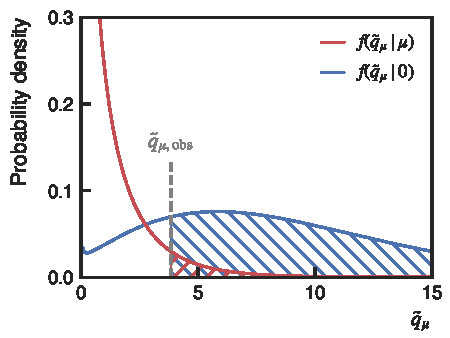
\includegraphics[width=\textwidth]{statistics/cls_high_sensitivity}
    \caption{}
  \end{subfigure}\hfill%
  \begin{subfigure}{0.46\textwidth}
    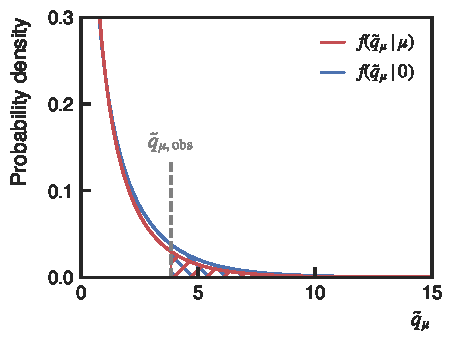
\includegraphics[width=\textwidth]{statistics/cls_low_sensitivity}
    \caption{}
  \end{subfigure}

  \caption{Bla}
\end{figure}

An example of
such a scenario is a counting experiment with a large expected number of
background events and small expected number of signal events.


If the observed number of events


, and in extreme cases completely exclude the signal-plus-background hypothesis.




. In extreme cases




Such spurious exclusions are of course expected, since the estimated confidence
intervals have an (approximate) coverage probability of $(1 - \alpha)$.






If the observed number of events is below the background expectation, . For extreme downward fluctuations




An example of such a scenario is a region with a large expected number of
background events



penalising






background expectation and





An example of
such a scenario










conservative in regions where there is little sensitivity to a signal.






The method introduced above








In particle physics, this method is slightly modified to counteract



This method of estimating upper limits on $\mu$ is perceived


This method of estimating upper limits is perceived to have .

approximate coverage probability of $(1 - \alpha)$


$(1 - \alpha)$.

This method addresses

In searches for new physics, a modified approach is adopted to derive upper
limits on the signal strength, which is referred to as the
\CLs~technique~\cite{Junk:1999kv,Read:2002hq}.





This method addresses spurious exclusions of signals to which an analysis






This method addresses

previous method (sometimes referred to as \CLsb)







In particle physics, a modified approach is adopted to derive upper limits on
the signal strength, which is referred to as the
\CLs~technique~\cite{Junk:1999kv,Read:2002hq}.

overcoverage


In particle physics, a modified approach is taken that yields more conservative
confidence intervals.









% until $p_\mu$ is equal to the chosen value of $\alpha$.


However, in particle physics






\vspace{5em}

Conventionally, upper limits are set at $\SI{95}{\percent}$ CL
($\alpha = 0.05$) in HEP. An empirical test statistic derived from the LRT is
defined according to


Conventionally, upper limits are set at $\SI{95}{\percent}$~CL
($\alpha = 0.05$) in HEP, although using a more conservative approach that will
be introduced shortly.


Using the asymptotic approximation, an iterative procedure can be employed to
find the value of $\mu$ such that
\begin{align*}
  \CLsb
  = 1 - \int_{\tilde{q}_{\mu, \text{obs}}}^{\infty} \mathrm{d}\tilde{q}_{\mu} \, f(\tilde{q}_{\mu} \mid \mu)
\end{align*}
is equal to \SI{95}{\percent}.



However, in particle physics a more conservative approach is taken to set upper
limits. The \CLs method


CLs method:

\begin{align}
  \text{CL}_\text{s+b} = \int^\infty_{q_\text{obs}} f(\tilde{q}_\mu \mid \mu) \, \mathrm{d}\tilde{q}_\mu \\
  \text{CL}_\text{b} = \int^\infty_{q_\text{obs}} f(\tilde{q}_\mu \mid 0) \, \mathrm{d}\tilde{q}_\mu
\end{align}


\begin{align}
  \text{CL}_\text{s} = \frac{\text{CL}_\text{s+b}}{\text{CL}_\text{b}}
\end{align}


\subsection{Treatment of Statistical Uncertainties on Background Rate
  Predictions}%
\label{sec:barlow_beeston}

The predicted background rate in a given bin $b$ of a channel $c$ is
determined from a finite sample of events, e.g.\ from MC simulation,
and thus does not directly correspond to the true expected rate. The
background rate estimates are subject to uncertainties that have to be
considered when performing inference, particularly when bins are only
sparsely populated with events.

This uncertainty is included in the likelihood function, employing the
method proposed by Barlow and Beeston~\cite{barlow1993}, by replacing
the expected background rate from the prediction using the finite
sample with the true expected rate that has to be simultaneously
inferred. In practice this is done by performing the substitution
$\nu_{cb} \rightarrow \gamma_{cb} \nu_{cb}$ that introduces new
nuisance parameters $\gamma_{cb}$ specifying the relative difference
between the predicted and true expected rates. Initially it was
proposed to introduce one such nuisance parameter for every background
source~\cite{barlow1993}, however, a simplified version proposed in
Ref.~\cite{conway2011} is used such that only the combined uncertainty
on the total background prediction is considered instead.

The $\gamma$ nuisance parameters are constrained by auxiliary
measurements using the observed samples of events entering the
bins. These measurements contribute terms of the form
\begin{align*}
  \pois(m_{cb} | \gamma_{cb} \tau_{cb})
  \qquad \text{with} \qquad
  \tau_{cb} = \frac{( \sum_i w_i )^2}{\sum_i w_i^2} = \text{const.}
\end{align*}
to the likelihood function~\cite{cranmer2012}, where the sums go over
all events contributing to bin $b$ in channel $c$ with event weights
$w_i$. This corresponds to a measurement of the effective number of
events based on the observed value $m_{cb}$, which is nominally equal
to $\tau_{cb}$\footnote{It should be noted that $m_{cb}$ are generally
  not integer-valued quantities and thus do not agree with the support
  of the Poisson distribution. Thus the factorial term in the Poisson
  PMF is replaced by the continuous gamma function to generalise the
  distribution to $\mathbb{R}^+$.}, from the finite sample.

This approach is based on the approximation of the \emph{compound
  Poisson distribution} (CPD) that describes the distribution of the
sum of a Poisson number of random weights with a \emph{scaled Poisson
  distribution} (SPD)~\cite{Bohm:2013gla}. The CPD describes the
distribution of rate predictions based on a finite sample of weighted
events and can be defined as
\begin{align*}
  X = \sum_{i = 1}^{N} W_i \quad \text{with} \quad N \sim \pois(\lambda) \quad \text{and} \quad \text{i.i.d.\ } W_i \text{ (independent of }N\text{)} \,\text{.}
\end{align*}
It can be approximated, see for example Ref.~\cite{Bohm:2013gla},
using a scaled Poisson distribution defined by
\begin{align*}
  \tilde{X} = s \cdot \tilde{N} \quad \text{with} \quad \tilde{N} \sim \pois(\tilde{\lambda})
\end{align*}
with
\begin{align*}
  s = \frac{\expect(W^2)}{\expect(W)} \qquad \tilde{\lambda} = \frac{\lambda \expect(W)^2}{\expect(W^2)}
\end{align*}
where $\expect(W)$ and $\expect(W^2)$ are the first and second moment
of the weight distribution. The Barlow-Beeston method makes the
assumption that the expectation values can be approximated by sample
averages such that
\begin{align*}
  s = \frac{\sum_i w_i^2}{\sum_i w_i} \qquad \tilde{\lambda} = \frac{\lambda}{n} \frac{(\sum_i w_i)^2}{\sum_i w_i^2}
\end{align*}
with sample size $n$. Comparing the equation for $\tilde{\lambda}$
with the constraint term entering the likelihood function illustrates
the connection to a measurement of the effective number of events. A
number of $\tilde{N}$ events contribute with equal weights given by
$s$ to the sum, thus $\tilde{N}$ can be referred to as an effective
number of events.

These relationships will be needed in the context of the statistical
interpretation of the results in~\Cref{sec:toys_global_observables}.


%%% Local Variables:
%%% mode: latex
%%% TeX-master: "../../phd_thesis"
%%% End:
